\documentclass{article}
\usepackage[polish]{babel}
\usepackage[T1]{fontenc}
\usepackage{amsmath}
\usepackage{amsfonts}
\usepackage{float}
\usepackage{graphicx} % Required for inserting images
\graphicspath{ {./images/} }

\title{Laboratorium 11 \\ Optymalizacja}
\author{Maciej Borowiec}
\date{18.06.2025}

\begin{document}

\maketitle

\section{Wprowadzenie}
Celem ćwiczenia było wykonanie dwóch zadań związanych z zagadnieniem optymalizacji. Pierwsze porównało spadek wzdłuż gradientu z metodą najmniejszych kwadratów dla układu równań liniowych, a drugie pokazało użycie metody największego spadku dla optymalizacji funkcji nieliniowej.

\section{Zadania}

\subsection{Zadanie 1.}
Zadanie polegało na rozwiązaniu zadania z laboratorium drugiego przy użyciu spadku wzdłuż gradientu i porównaniu otrzymanych wyników. Należało zaimplementować funkcję rozwiązującą zagadnienie, używając spadku wzdłuż gradientu ze stałą uczącą wyznaczoną z najmniejszej i największej wartości własnej macierzy $A^TA$ ($\alpha = \frac{1}{\lambda_{min} + \lambda_{max}}$). W poniższej tabeli znajduje się porównanie tych metod.
\begin{table}[h!]
    \centering
    \begin{tabular}{|c|c|c|c|c|c|c|}
        \hline
        Metoda & TP & TN & FP & FN & Dokładność & Czas obliczeń \\
        \hline
        Najmniejszych kwadratów & $58$ & $194$ & $6$ & $2$ & $96.923\%$ & $0.000169$s \\
        Spadku wzdłuż gradientu & $38$ & $200$ & $0$ & $22$ & $91.538\%$ & $0.010647$s \\
        \hline
    \end{tabular}
    \caption{Porównanie metod dla rozwiązania zagadnienia z laboratorium 2.}
    \label{table}
\end{table}
\\
Jak widać w danej tabeli (Tabela 1), dla tego problemu lepszą metodą okazała się metoda najmniejszych kwadratów. Dla tej metody dokładność jest zauważalnie większa. Metoda spadku wzdłuż gradientu nie zanotowała żadnych przypadków fałszywie dodatnich, ale za to uzyskała znacznie więcej przypadków fałszywie ujemnych. Czasowo też metoda najmniejszych kwadratów wyszła znacznie lepiej. Jest to zgodne z teorią, gdyż metoda najmniejszych kwadratów ma złożoność czasową równą $O(nm^2 + m^3)$, a dla metody spadku wzdłuż gradientu wynosi ona $k*O(nm)$ ($n,m$ - wymiary macierzy, $k$ - liczba iteracji w metodzie spadku wzdłuż gradientu). Macierz ma wymiary $300\times31$, a iteracji wykonano $5000$ (dla mniejszej liczby iteracji dokładność była mniejsza od 90\%), dlatego czasy obliczeń są zgodne z teorią.

\subsection{Zadanie 2.}
W tym zadaniu należało wyznaczyć najkrótszą ścieżkę od punktu startowego do końcowego dla robota, używając metody największego spadku. Mamy dane:
\begin{itemize}
\item $x^{(0)}, x^{(1)}, ..., x^{(n)}$ ($x^{(i)} \in \mathbb{R}^2$) - punkty ścieżki jako argumenty funkcji kosztu, gdzie $x^{(0)}$ i $x^{(n)}$ to niezmienne punkty startu i końca ścieżki
\item $r^{(1)}, r^{(2)}, ..., r^{(k)}$ ($r^{(i)} \in \mathbb{R}^2$) - punkty symbolizujące przeszkody
\end{itemize}
W celu optymalizacji ścieżki robota użyjemy zadanej funkcji kosztu:
$$F(x^{(0)},x^{(1)},...,x^{(n)}) = \lambda_1\sum_{i=0}^n\sum_{j=1}^k\frac{1}{\epsilon+||x^{(i)}-r^{(j)}||^2_2} + \lambda_2\sum_{i=0}^{n-1}||x^{(i+1)}-x^{(i)}||^2_2$$
gdzie:
\begin{itemize}
\item $\lambda_1$ określa wagę składnika zapobiegającego zbytniemu zbliżaniu się do przeszkody
\item $\lambda_2$ określa wagę składnika zapobiegającego tworzeniu bardzo długich ścieżek
\item $\epsilon$ zapobiega dzieleniu przez 0
\end{itemize}

\subsubsection{Wyznaczenie gradientu $\nabla F$ dla funkcji $F$}
Należało wyznaczyć gradient dla funkcji kosztu $F$. Chcemy, żeby punkty $x^{(0)}$ i $x^{(n)}$ były stałe, zatem względem nich gradient zostanie wyzerowany. Otrzymujemy, więc:
$$\nabla F = [0, \frac{\partial F}{\partial x^{(1)}}, \frac{\partial F}{\partial x^{(2)}}, ..., \frac{\partial F}{\partial x^{(n-1)}}, 0]$$
Do obliczenia gradientu potrzebujemy zatem obliczyć $\frac{\partial F}{\partial x^{(i)}}, i=1,2,...,n-1$. Zdefiniujmy:
\begin{equation}
    S_1 = \sum_{i=0}^n\sum_{j=1}^k\frac{1}{\epsilon+||x^{(i)}-r^{(j)}||^2_2}
\end{equation}
\begin{equation}
    S_2 = \sum_{i=0}^{n-1}||x^{(i+1)}-x^{(i)}||^2_2
\end{equation}
Wtedy:
$$F = \lambda_1S_1 + \lambda_2S_2 \implies \frac{\partial F}{\partial x^{(i)}} = \lambda_1\frac{\partial S_1}{\partial x^{(i)}} + \lambda_2\frac{\partial S_2}{\partial x^{(i)}}$$
Obliczmy pochodną cząstkową dla równania (1):
$$\frac{\partial S_1}{\partial x^{(i)}} = \frac{\partial}{\partial x^{(i)}}(\sum_{l=0}^n\sum_{j=1}^k\frac{1}{\epsilon+||x^{(l)}-r^{(j)}||^2_2})$$
Możemy pominąć składniki bez zmiennej $x^{(i)}$:
$$\frac{\partial S_1}{\partial x^{(i)}} = \frac{\partial}{\partial x^{(i)}}(\sum_{j=1}^k\frac{1}{\epsilon+||x^{(i)}-r^{(j)}||^2_2})$$
$$\frac{\partial S_1}{\partial x^{(i)}} = -2\sum_{j=1}^k\frac{x^{(i)}-r^{(j)}}{(\epsilon+||x^{(i)}-r^{(j)}||^2_2)^2}$$
Obliczmy też pochodną cząstkową dla równania (2):
$$\frac{\partial S_2}{\partial x^{(i)}} = \frac{\partial}{\partial x^{(i)}}(\sum_{l=0}^{n-1}||x^{(l+1)}-x^{(l)}||^2_2)$$
$$\frac{\partial S_2}{\partial x^{(i)}} = \frac{\partial}{\partial x^{(i)}}(||x^{(i)}-x^{(i-1)}||^2_2 + ||x^{(i+1)}-x^{(i)}||^2_2)$$
$$\frac{\partial S_2}{\partial x^{(i)}} = 2(x^{(i)}-x^{(i-1)}) - 2(x^{(i+1)}-x^{(i)})$$
$$\frac{\partial S_2}{\partial x^{(i)}} = 2(-x^{(i+1)}+2x^{(i)}-x^{(i-1)})$$
Ostatecznie:
$$\frac{\partial F}{\partial x^{(i)}} = -2\lambda_1\sum_{j=1}^k\frac{x^{(i)}-r^{(j)}}{(\epsilon+||x^{(i)}-r^{(j)}||^2_2)^2} + 2\lambda_2(-x^{(i+1)}+2x^{(i)}-x^{(i-1)})$$

\subsubsection{Opis algorytmu}
Zaimplementowany algorytm wygląda następująco:
\begin{enumerate}
\item Inicjalizujemy punkty startowe $x^{(i)}$ (w tym punkt startowy i końcowy) oraz listę do przechowywania wartości funkcji kosztów w danej iteracji. Dodajemy do listy kosztów wartość funkcji kosztu dla punktów początkowych.
\item Obliczamy gradient funkcji dla danych punktów $x^{(i)}$.
\item Znajdujemy długość kroku używając metody złotego środku - w tym celu zakładamy, że funkcja $F$ jest unimodalna (mimo, że w rzeczywistości tak nie jest).
\item Aktualizujemy punkty $x^{(i)}$ zgodnie z długością kroku i gradientem.
\item Dodajemy do listy kosztów wartość funkcji kosztu dla zaktualizowanych punktów $x^{(i)}$.
\item Wracamy do kroku 2. i powtarzamy czynności aż wartość bezwzględna różnicy kolejnych kosztów jest wystarczająco mała lub dojdziemy do limitu iteracji.
\end{enumerate}

\subsubsection{Przedstawienie otrzymanych wyników}
Należało znaleźć najkrótszą ścieżkę robota, używając algorytmu z zadanymi parametrami:
\begin{itemize}
\item $n=20, k=50$
\item $x^{(0)} = [0,0], x^{(n)} = [20,20]$
\item $r^{(i)} \sim \mathcal U(0,20) \times \mathcal U(0,20)$
\item $\lambda_1 = \lambda_2 = 1$
\item $\varepsilon = 10^{-13}$
\item liczba iteracji = $400$
\end{itemize}
Obliczenia należało przeprowadzić dla pięciu różnych, losowych inicjalizacji punktów początkowych (za wyjątkiem punktu startowego i końcowego ścieżki). Poniżej przedstawiony został wykres funkcji kosztu w zależności od danej iteracji oraz tabela zestawiająca koszty początkowe z kosztami końcowymi.
\begin{figure}[H]
    \centering
    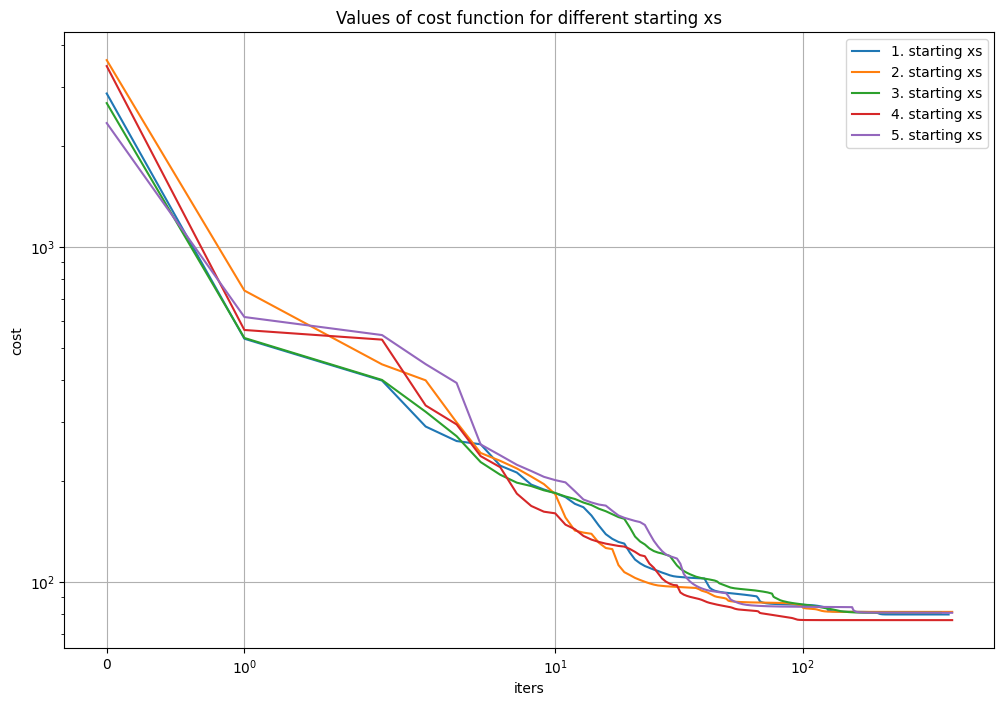
\includegraphics[width=0.95\textwidth]{1}
    \caption{Wykres wartości funkcji kosztu w zależności od iteracji}
    \label{fig:mesh}
\end{figure}
\begin{table}[h!]
    \centering
    \begin{tabular}{|c|ccccc|}
        \hline
        Punkty startowe & 1. & 2. & 3. & 4. & 5. \\
        \hline
        Koszt początkowy & $2868.114$ & $3607.629$ & $2684.610$ & $3462.098$ & $2340.272$ \\
        Koszt końcowy & $79.815$ & $81.243$ & $80.731$ & $76.775$ & $80.745$ \\
        \hline
    \end{tabular}
    \caption{Zestawienie kosztów początkowych i końcowych dla zadanych zbiorów punktów startowych}
    \label{table}
\end{table}
Z danego wykresu (Rysunek 1) i tabeli (Tabela 2) widać, że metoda największego spadku dokonała dobrej optymalizacji funkcji zadanej w tym problemie. Udało się zmniejszyć koszt początkowy z kilku tysięcy do kilkudziesięciu dla każdego zbioru punktów startowych. Największa redukcja kosztu nastąpiła dla pierwszego kroku, a dla dalszych było już to zależne od startowych punktów. Można jednak zauważyć, że dla około setnej iteracji koszt zaczął się zmniejszać w bardzo małym stopniu.
\\\\
Przedstawmy również przykładową ścieżkę przed i po optymalizacji.
\begin{figure}[H]
    \centering
    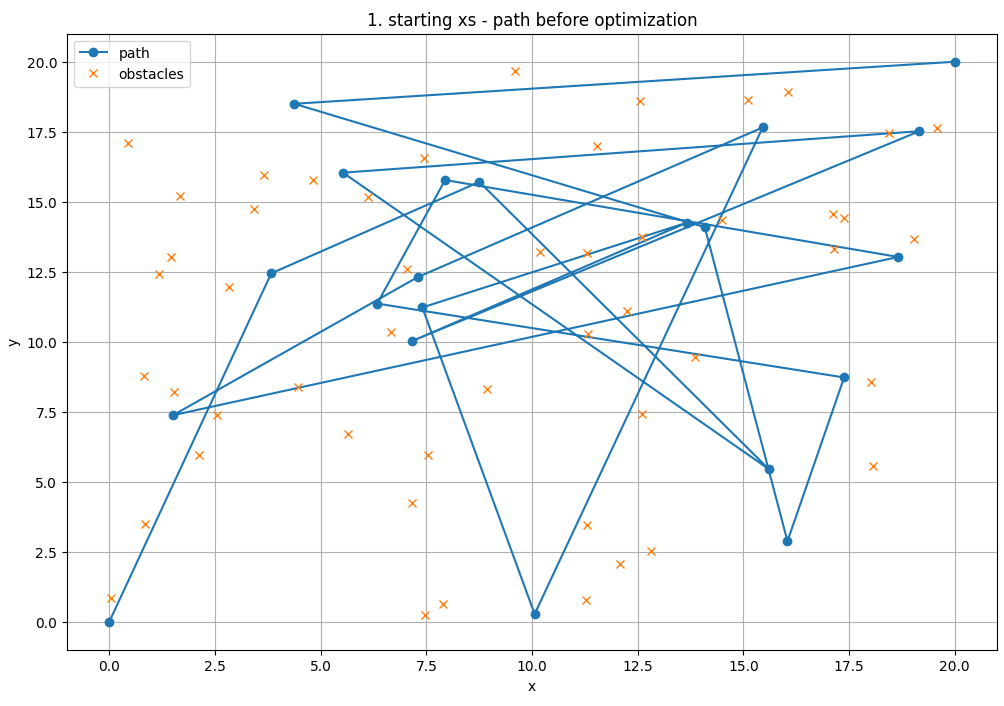
\includegraphics[width=0.95\textwidth]{2}
    \caption{Przykładowa ścieżka przed optymalizacją}
    \label{fig:mesh}
\end{figure}
\begin{figure}[H]
    \centering
    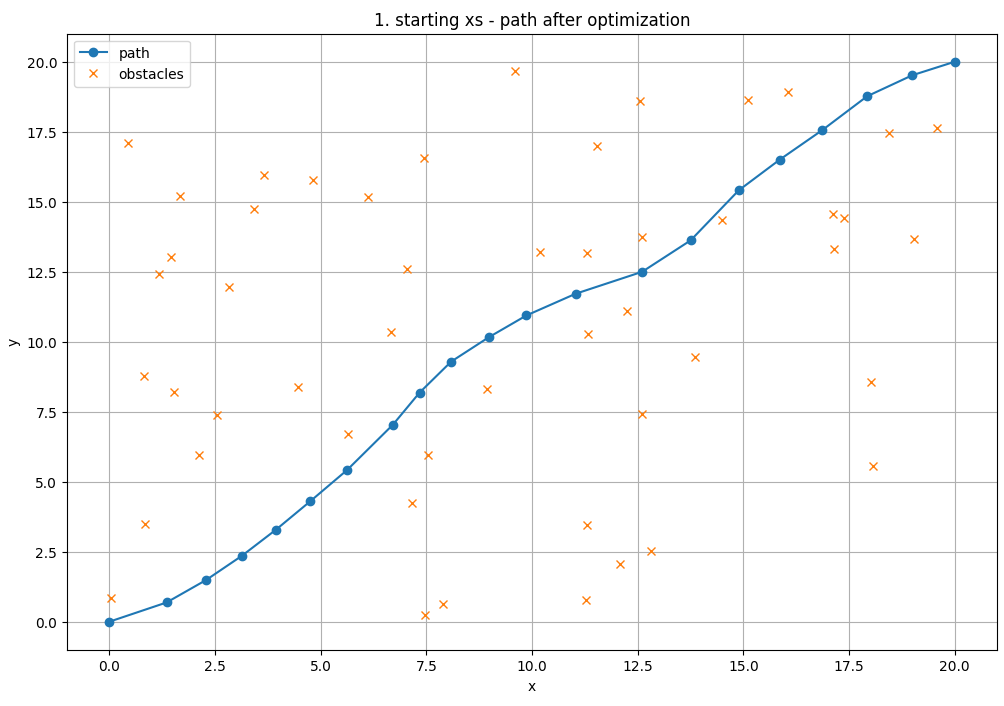
\includegraphics[width=0.95\textwidth]{3}
    \caption{Przykładowa ścieżka po optymalizacji}
    \label{fig:mesh}
\end{figure}
Jak widać z podanych rysunków (Rysunek 2, 3), znaleziona ścieżka, używając optymalizacji, jest znacznie lepsza od startowej, losowej ścieżki.

\section{Podsumowanie}
Zadania z tego laboratorium pokazały metody rozwiązywania zadań z zagadnienia optymalizacji.
\\
Zadanie 1. pokazało, że nie należy zawsze, bezmyślnie, stosować metod spadku wzdłuż gradientu dla każdego zadania związanego z optymalizacją. Dla prostych układów równań (np. liniowych), szczególnie dla niewielkiej liczby danych i parametrów, lepiej poradzą sobie prostsze metody. W tym przypadku metoda najmniejszych kwadratów okazała się szybsza i dokładniejsza.
\\
Zadanie 2. pokazało zastosowanie gradientu do optymalizacji funkcji nieliniowej. Pokazało, że jeśli jesteśmy w stanie obliczyć gradient funkcji kosztu, to możemy go użyć z dużym sukcesem do optymalizacji. Nie było to jednak bez swoich wad. Funkcja kosztu i jej gradient były na tyle skomplikowane, że wykonanie obliczeń dla wszystkich początkowych zbiorów punktów zajęło w sumie kilka minut.
\section{Bibliografia}
\begin{itemize}
\item Materiały zamieszczone wraz z zadaniem
\end{itemize}

\end{document}
